\documentclass{bioinfo}
\copyrightyear{2015} \pubyear{2015}

\access{Advance Access Publication Date: Day Month Year}
\appnotes{Manuscript Category}

\begin{document}
\firstpage{1}

\subtitle{Subject Section}

\title[short Title]{Model Sub-tissue Morphological Components in mass spectrometry imaging data Using Dirichlet Gaussian Mixture Model}
\author[Sample \textit{et~al}.]{Corresponding Author\,$^{\text{\sfb 1,}*}$, Co-Author\,$^{\text{\sfb 2}}$ and Co-Author\,$^{\text{\sfb 2,}*}$}
\address{$^{\text{\sf 1}}$Department, Institution, City, Post Code, Country and \\
$^{\text{\sf 2}}$Department, Institution, City, Post Code,
Country.}

\corresp{$^\ast$To whom correspondence should be addressed.}

\history{Received on XXXXX; revised on XXXXX; accepted on XXXXX}

\editor{Associate Editor: XXXXXXX}

\abstract{\textbf{Motivation:} Text Text Text Text Text Text Text Text Text Text Text Text Text
Text Text Text Text Text Text Text Text Text Text Text Text Text Text Text Text Text Text Text
Text Text Text Text Text Text Text Text Text Text Text Text Text Text Text Text Text Text Text
Text Text Text Text Text Text
Text Text Text Text Text.\\
\textbf{Results:} Text  Text Text Text Text Text Text Text Text Text  Text Text Text Text Text
Text Text Text Text Text Text Text Text Text Text Text Text Text  Text Text Text Text Text Text\\
\textbf{Availability:} Text  Text Text Text Text Text Text Text Text Text  Text Text Text Text
Text Text Text Text Text Text Text Text Text Text Text Text Text Text  Text\\
\textbf{Contact:} \href{name@bio.com}{name@bio.com}\\
\textbf{Supplementary information:} Supplementary data are available at \textit{Bioinformatics}
online.}

\maketitle

\section{Introduction}



Mass spectrometry imaging experiment typically collects 100-10000 Da m/z, which generates almost 20000 ion images for a single tissue section. Currently, complete mining of such data requires the user to click through each image and look for distributions that may correlate to the morphology of the sample analyzed. This is very laboursome and subject. \\
\\
Though mannually data mining is widely used, unsupervised data processing techniques are also used in imaging laboratory. \\
\\
Peak picking from a mean spectrum can pick out high abundant ions, while the ions co-localized in a small area may missed. Moreover, the picked high abundant ions may not have the morphological information and distributed globally homogeneous instead.\\
\\
For dimension reduction method, such as PCA, ions with high loadings were considerated as "important ions". However, ions with high loadings represent globally high variance, which are not nessacerily the ions which correlated to the morphology of sample.\\
\\
Multivariate segmentation methods such as spatial k-means and spatial centroid segmentation, are also popular methods to explore the similarity and spatial correlation of pixels. Spatial K-means segmentation is not able to select ions, while spatial centroid segmentation can select important ions related to each segments. However the segmentation results of these multivariate menthods can not represent every single ion spatial distribution morphology, which is shown in Figure 1 and Figure 2. Moreover, sometimes the "spatial mask" of spatial K-means and spatial centroid segmentation is difficult to interprate, as shown in Figure 2.\\
\\  

Since single ion image is of great interest of mining and the signal of single ion image would be covered by multivariate analysis,  univariate analysis should be performed. To our best knowledge, there're two approaches to model single ion image. \\
\\ 

---homegeneity index, which used a new texture anaysis to evaluate the level of homogeneity of single ion distribution.\\
---structured and non-structured index, which used a new form of entropy of evaluate the level of structuredness of ion images to select low abundant but structured ions\\

Hoever, none of these methods can model the spatial morphology of single ion image.\\

In this paper, we proposed a new Dirichlet Gaussian Mixture model which incoorperates spatial dependence to model single ion spatial distribution. In this model, the number of Gaussian components (spatial sub-structure) was atomantically decided. It's straight forward to interpret the results of the model since it's single ion.\\

importance to class comparison.
  \citep{Bag01} wants to know about
{\ldots}{\ldots} text follows.
\begin{equation}
\sum \text{\it x}+ \text{\it y} =\text{\it Z}\label{eq:01}\vspace*{-10pt}
\end{equation}
\begin{figure}[b!]
    \centering
	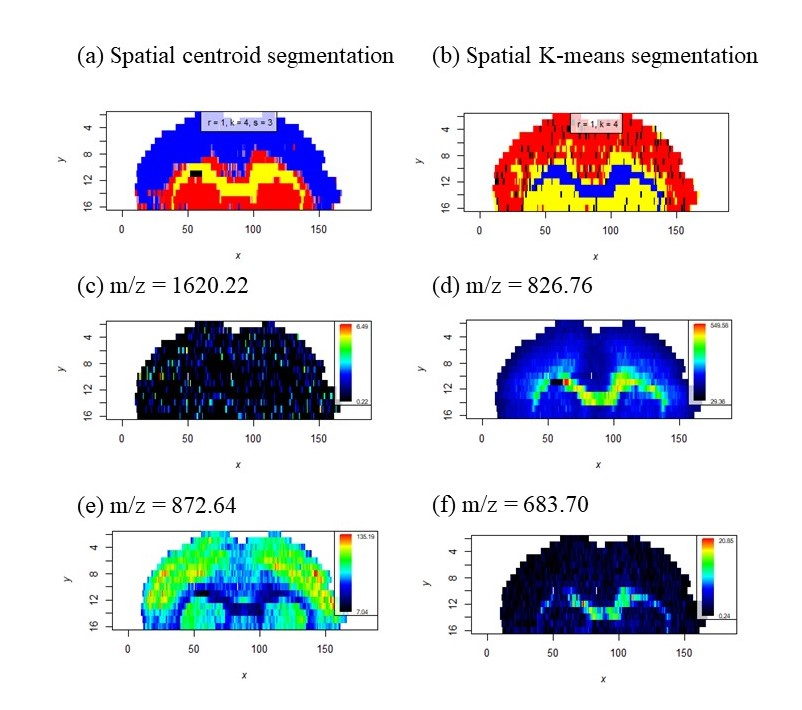
\includegraphics[width=0.4\textwidth]{figure1.jpg}
    \caption{ MSI data of a mouse brain tissue. (a) spatial centroid segmentation results of 433 $m/z$s; (b) spatial K-means segmentation results of 433 $m/z$s; (c-f) sing ion image of $m/z$ 1620.22, 826.76, 872.64 and 683.70 respectively.}
    \label{fig:figure1}
\end{figure}
\citealp{Boffelli03} might want to know about text text text
text\vspace*{1pt}


\begin{figure}[b!]
    \centering
	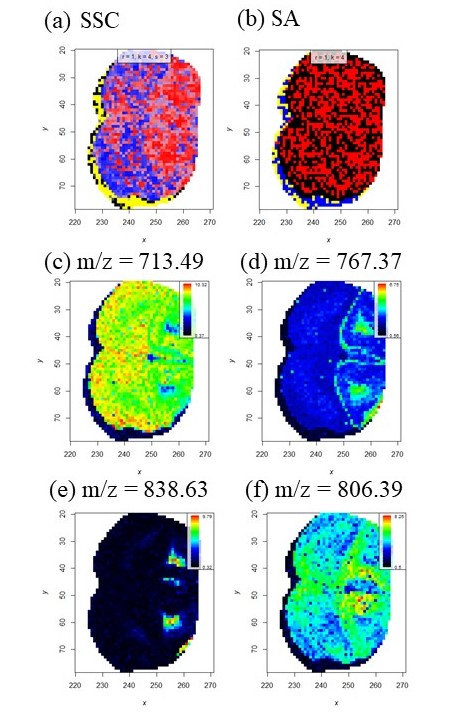
\includegraphics[width=0.35\textwidth]{figure2.jpg}
    \caption{MSI data of a mouse brain tissue. (a) spatial centroid segmentation results of 60 $m/z$s; (b) spatial K-means segmentation results of 60 $m/z$s; (c-f) sing ion image of $m/z$ 713.49, 767.37, 38.63 and 806.39 respectively.}
    \label{fig:figure2}
\end{figure}
\citealp{Boffelli03} might want to know about text text text
text\vspace*{1pt}


\section{Methods}

$x^i, i = (1,2,...,N)$, denotes the ion intensity at pixel $i$.\\
$\pi^i={\pi^i_1,..., \pi^i_K}$ denotes the prior probability of each component the $i_{th}$ pixel belongs to.\\
$z^i={z^i_1,...,z^i_K}$ denotes the discrete label of the $i_{th}$ pixel.\\
$$z^i_j=\left\{\begin{matrix}
1 \textrm{ if pixel i belongs to component j}\\ 
0 \textrm{ otherwise} 

\end{matrix}\right.$$

$$p(x^i)=\sum_{j=1}^{K}\pi^i_jp(x^i|\theta_j)$$

$$p(x^i)=\sum_{j=1}^{K}\pi^i_jp(x^i|\theta_j)p(\theta_j|\theta_{T_j})$$

$$p(x^i)=\sum_{j=1}^{K}\pi^i_jp(x^i|\theta_j)p(\theta_j|\theta_{T_j}+\gamma \theta_{T_j}')$$

$$p(x^i|\theta_j)=\frac{1}{(2\pi)^{1/2}}exp(-\frac{1}{2}(x^i-\mu_j)^2\sigma_j^{-1})$$

The log-likelihood is:

$$L(\Theta )=\sum_{i=1}^{N}log{\sum_{j=1}^{K}\pi^i_jp(x^i|\theta_j)}+logp(\Pi )$$

The discrete label $z^i_j$ is a random variable following a multinomial distribution with $M$ realizations.\\

$$p(z^i|\xi ^i)=\frac{M!}{\prod_{j=1}^{K}(z^i_j)!}\prod_{j=1}^{K}(\xi ^i_j)^{z^i_j}$$

in which $(\xi ^i_j)\ge0$ and $\sum_{j=1}^{K}\xi ^i_j=1$

The Dirichlet process id defined as:\\

$$p(\xi ^i|\alpha^i)=\frac{\Gamma (\sum_{j=1}^{K}\alpha^i_j)}{\prod_{j=1}^{K}\Gamma (\alpha^i_j)}\prod_{j=1}^{K}(\xi^i_j)^{(\alpha^i_j-1)}$$

In which, $\alpha^i (\alpha^i>0)$ is the vector of Dirichlet parameters.

$$p(z^i|\alpha^i)=\frac{M!\Gamma (\sum_{j=1}^{K}\alpha^i_j)}{\prod_{j=1}^{K}(z^i_j)!\Gamma (\sum_{j=1}^{K}(\alpha^i_j+z^i_j))}\prod_{j=1}^{K}{\frac{\Gamma(\alpha^i_j+z^i_j)}{\Gamma(\alpha^i_j)}}$$

$$\pi^i_j=p(z^i_j=1|\alpha_i)=\frac{\alpha^i_j}{\sum_{k=1}^{K}\alpha^i_k}$$

Incorporate the spatial dependence:\\

The posterior probability at iteration $t$ is given by:


$$y^{i(t)}_j=\frac{\pi^i_jp(x^i|\theta_j)}{\sum_{k=1}^{K}\pi^i_kp(x^i|\theta_k)}$$

To introduce the relationship between neighboring pixels, define\\

$$\bar{y}^{i}_j=\frac{1}{\sum_{m\subseteq N^i}d^i_m}\sum_{m\subseteq N^i}d^i_{m}y^{m(t-1)}_j$$

In which, $d^i_m$ is the combination of spatial distance and spectrum similarity of two neighboring pixels, which can be written as:\\

$$d^i_m=exp(\frac{(i-m)^2}{\sigma_1})exp(\frac{(S_i-S_m)^2}{\sigma_2})$$

The new Dirichlet distribution is defined as:\\
$$p(\xi ^i|\alpha^i)=\frac{\Gamma (\sum_{j=1}^{K}\alpha_j^2 \bar{y}^{(i)\beta}_j)}{\prod_{j=1}^{K}\Gamma (\alpha_j^2 \bar{y}^{(i)\beta}_j)}\prod_{j=1}^{K}(\xi^i_j)^{(\alpha_j^2 \bar{y}^{(i)\beta}_j-1)}$$

Therefore, the error function $E(\Theta )$ is:
$$E(\Theta )=-\sum_{i=1}^{N}\sum_{j=1}^{K}y^{i(t)}_j\{log(\alpha_j^2\bar{y}^{(i)\beta}_j)-log(\sum_{k=1}^{K}\alpha_k^2\bar{y}^{(i)\beta}_k)-\frac{1}{2}log(2\pi)-\frac{1}{2}log(\sigma_j)-\frac{1}{2}(x^i-\mu_j)^2\}$$

In which, $\Theta =(\mu_j, \sigma_j, \alpha_j, \beta)$\\

The objective is to $min_\Theta E(\Theta)$.\\


In the M step,
$$\Theta ^{(t+1)}=\Theta ^{(t)}-\eta \bigtriangledown E(\Theta ^{(t)})$$

In which $eta$ is the learning step. All $\bigtriangledown E(\Theta ^{(t)})$ has closed form and are subject to the constrains.



\begin{figure}[b!]

	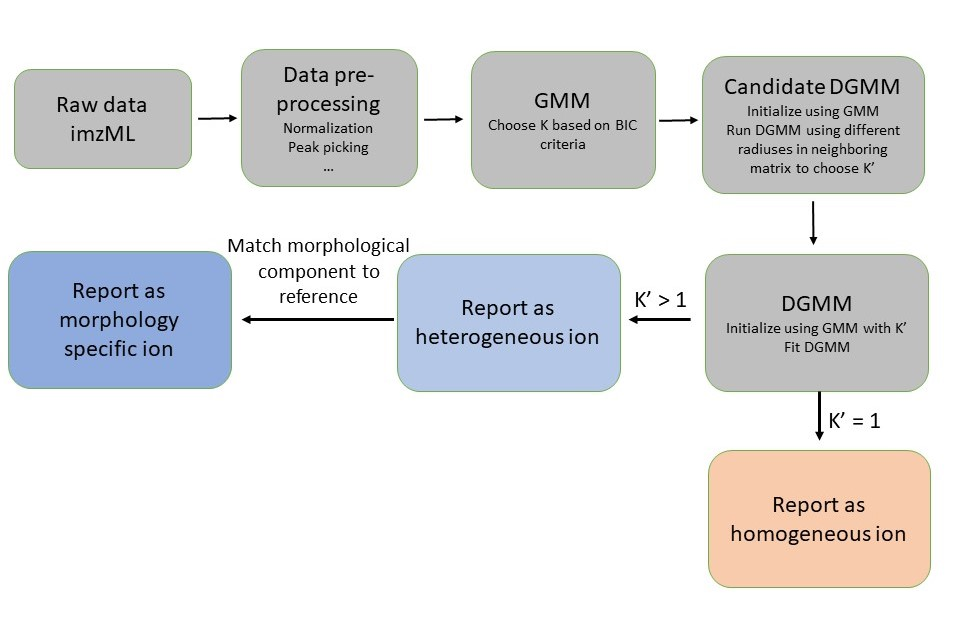
\includegraphics[width=0.5\textwidth]{figure3.jpg}
    \caption{flow chat sketch}
    \label{fig:figure3}
\end{figure}
\citealp{Boffelli03} might want to know about text text text
text\vspace*{1pt}




\section{Datasets}

\subsection{Simulated Data}
We simulated MSI datasets using function as below:
$$Y_{i}=\mu_{k(i)}+ \phi_i + \epsilon_i $$
$$ \phi_i  \sim ICAR (\tau^2, W) $$
in which $Y_i$ is the intensity oof pixel $i$, $\mu_{k(i)}$ the mean intensity of sub-tissue morphological component $k$ pixel $i$ belongs to, $\phi_i$ the spatial auto-correlation term and $\epsilon_i$ the nosie of pixel $i$. $\epsilon_i$ follows inttrisinc auto-correllation with variance $tau^2$ and $W$ as neighboring matirx.




In the first dataset we simulated, all MSI images have identical morphologies but different noise levels. As shown in Fig XXXXX, All MSI have three morphological components: circle, triangle and the rest of image and the mean intensities of three morphological cmponents are 100, 225, 150 respectively. The noise level varies from 5\% of mean intensity to 32\% of mean intensity. The variance for spatial auto-correlation is 25.



The second simulated data has 40 images or m/zs in total and every 10 m/zs have identical morphologies but different mean intensities for each morphological component. As shown in Fig XXXX, m/z 1-10 have three morphological components: circle, triangle and the rest of image, m/z 11-20 have two morphological components: triangle and the rest of image, m/z 21-30 have two morphological components: circle and the rest of image and m/z 31-40  have homogenouse ion spatial distribution.

\subsection{Saline and CPG preconditioned mouse brain}
CpG is ann unmethylated oligodeoxynucleotide that has been shown to stimulate the toll-like receptor 9 and induce neuroprotection against ischemic damage. To estimate the metabolic changes on brains caused by CpG preconditioning, brain tissue sections of saline (control) and CpG preconditioned mice were collected and analyzed by nano-MSI experiment using a Thermo LTQ-orbitrap instrument via positive mode. The spatial resolution is approximately 40 $\times$ 200 $\mu$m and the mass range is 100-1500 Da. The original MSI data are in RAW format and converted to NetCDF format using Xcalibur software before read by Cardinal.
\subsection{Amyotrophic lateral sclerosis mouse brain}
Amyotrophic lateral sclerosis is a neurodegenerative disease, 20\% of which is caused by mutations of SOD1. Mice who expressing a human ALS mutation, Cu-Zm superoxide dismutase 1 become symptomatic after ~130 days. Brain tissue sections of ALS mice and their non-SOD1/YFP littermates on day 150 were collected and analyzed by MALDI-MSI experiment using a solariX 9.4 T FTICR
(Bruker Daltonics, Billerica, MA, USA) instrument via positive mode. The spatial resolution is 100 $\mu$m and the mass range is 609.44-1400 Da. MALDI-MSI data were converted to imzML format before further processing using R.













\section{Results and Discussion}
In this section, we will first evaluate the performance of the proposed method in terms of estimation accuracy using simulated datasets and examinate the performace of the proposed model to exract the morhological component from single ion images. Then we will discuss the potential applications of the proposed model in biomarker discovery, tissue classification and class comparison.







\begin{table}[!t]
\processtable{This is table caption\label{Tab:01}} {\begin{tabular}{@{}llll@{}}\toprule head1 &
head2 & head3 & head4\\\midrule
row1 & row1 & row1 & row1\\
row2 & row2 & row2 & row2\\
row3 & row3 & row3 & row3\\
row4 & row4 & row4 & row4\\\botrule
\end{tabular}}{This is a footnote}
\end{table}



\begin{figure}[b!]
    \centering
	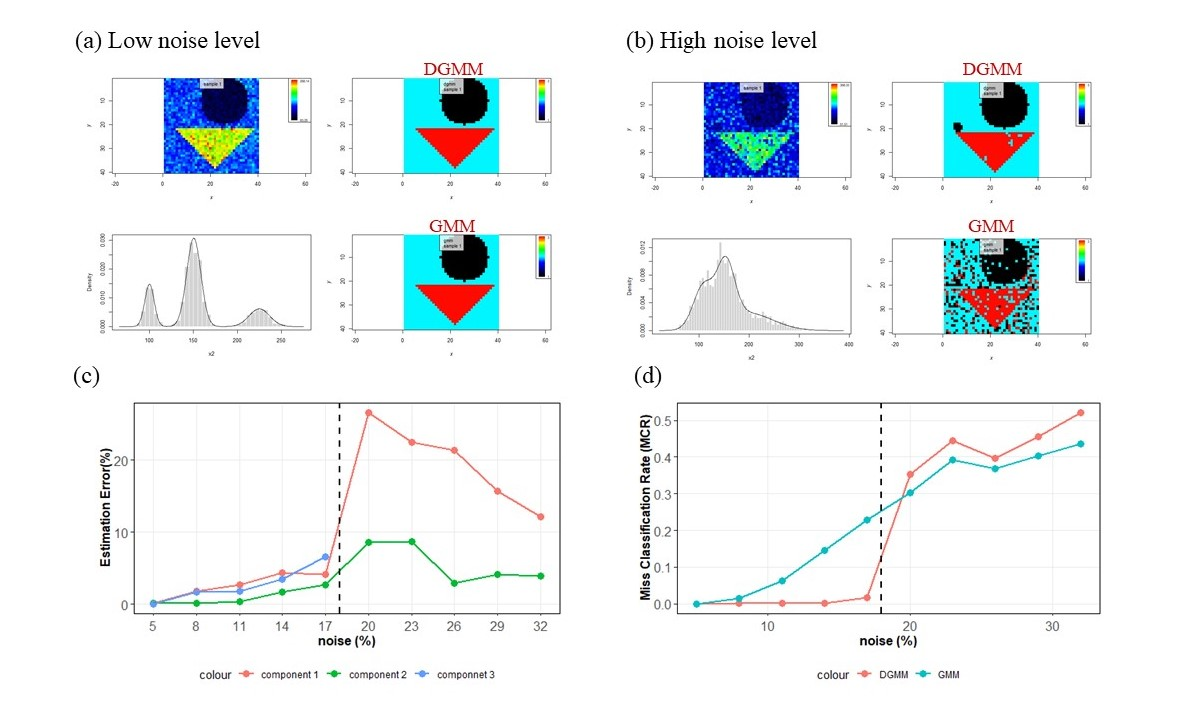
\includegraphics[width=0.6\textwidth]{figure4.jpg}
    \caption{Performance of DGMM on simulated dataset. (a) ion image (upper left), results of DGMM (upper right), histogram of ion itensities (lower left) and results of GMM(lower right) for low noise level data; (b) ion image (upper left), results of DGMM (upper right), histogram of ion itensities (lower left) and results of GMM(lower right) for high noise level data; (c) plot of estimation error of mean intensity of each morphological componnet vs noise level; (d) plot of misclassification rate vs noise level}
    \label{fig:figure4}
\end{figure}
\citealp{Boffelli03} might want to know about text text text
text\vspace*{1pt}



\subsection{Model performance}

As shown in Fig XXXXX, for low noise level dataset, both GMM and DGMM can report the correct number of morphological components and have very low estimation error of the mean intensity of each morphological component and very low error of misclassifying pixels to morphological components. As the noise level increases, the morphological component image generated by GMM becomes very noise and the misclassificatin rate increases rapidly. However GMM model has much lower estimation error of the mean intensitiy of each component and misclassification rate comparing to GMM before noise level of 20\% of mean. When noise level is above 20\% of mean, the reported number of morphological components are not correct. The performance on reporting the correct number of morphological components dependes on how distinguishable these components are. In general, for higher fold changes among mean intensities of components ans lower noise level, DGMM have better performace. In this case, the mean intensity of the background component,  circle component and triangle component have geometric 1.5 fold change and the noise tolerance is 20\%.


\begin{figure}[b!]
    \centering
	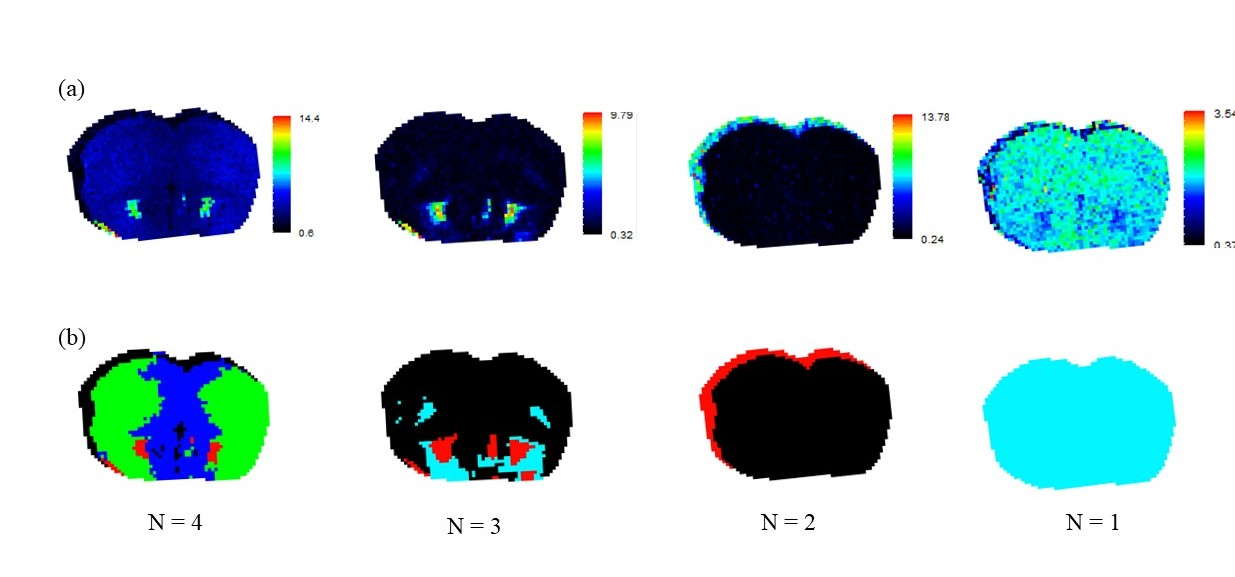
\includegraphics[width=0.8\textwidth]{figure5.jpg}
    \caption{Results of morpology modeled by DGMM (b) and the corresponding ion images (a)}
    \label{fig:figure5}
\end{figure}
\citealp{Boffelli03} might want to know about text text text
text\vspace*{1pt}

\subsection{Select Morphological Specific Ions}
\subsubsection{Identify ion of a heterogeneous distribution or homogeneous distribution}
A critical important task in MSI data analysis is to identify $m/z$ that have a heterogeneous distribution. $m/z$ of a heterogeneous distribution is usually related to anatomic structure of tissue or lessions, thus it's of great interest of further study. On the other hand, it's also important to evaluate whether ion has homogeneous distribution when it comes to drug delivery in clinical study. Although methods such as entropy analysis, texture analysis and morphometric analysis have been utilized to identify whether a $m/z$ has homogeneous distribution, none of them is able to provide the further information of spatial heterogeniety of each $m/z$. The proposed method can not only evaluate whether  a $m/z$ has homogeneous distribution and also provide the information of how many morphological components it has and the proportion and location of each components. (As shown in Fig XXXXXX) One can customize the minimum proportion of morphological components to ignore small hot ares based on respective research goal.



\subsubsection{Identify ion having a specific morphological component}
Identifying $m/z$ of a spatial pattern related to a specific area, which can be either an anatomic structure or an area of interest, is helpful to understand the molecular signisture and potential pathways of sub-tissue structures. Using correlation coefficient between ion image of a $m/z$ and binary matrix indicating a specific area is the most commonly used method to identify $m/z$ co-localized in this area. It's fast and reliable when the ion is only depressed or over expressed in the specific area. However when the ion has multiple morphological components, using correlation coefficient is not able to identify these $m/z$s. Fig XXXXX shows that the correlation of ion image of $m/z=XX$ is -0.51, which is comparatively low and similar to the correlation coefficient of ion image of $m/z=XX$. While we can see from the ion images that $m/z=XXX$ has a more clear morphology of segment showing in Fig XXX(a). In this paper, we fit DGMM on ion images of distinct $m/z$s first, then match each morphological component to the segment showing in FigXXXX and select the morphological componnet of the highest matching score. The morphological component of highest matching score of 0.36 in ion image of $m/zXXX$ is the red area. The morphological component colored in black  in ion image of $m/zXXX$ has a matching score of 0.78, which is distinguished from ion image of $m/z XXX$.

\begin{figure}[b!]
    
	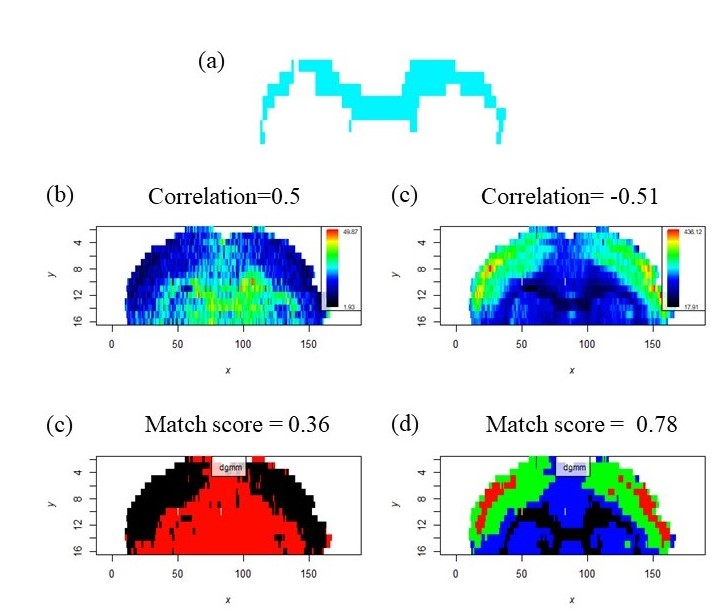
\includegraphics[width=0.5\textwidth]{figure6.jpg}
    \caption{(a) one segement generated by spatial centroid segmentation using 433 $m/z$s which looks like corpus collarium; (b) ion image of $m/z$ XXX; (c) ion image of $m/z$ XXX; (d) morphological component modeled by DGMM; }
    \label{fig:figure6}
\end{figure}
\citealp{Boffelli03} might want to know about text text text
text\vspace*{1pt}


\subsection{Clustering $m/z$s with similar spatial patterns}


\begin{figure}[b!]
    
	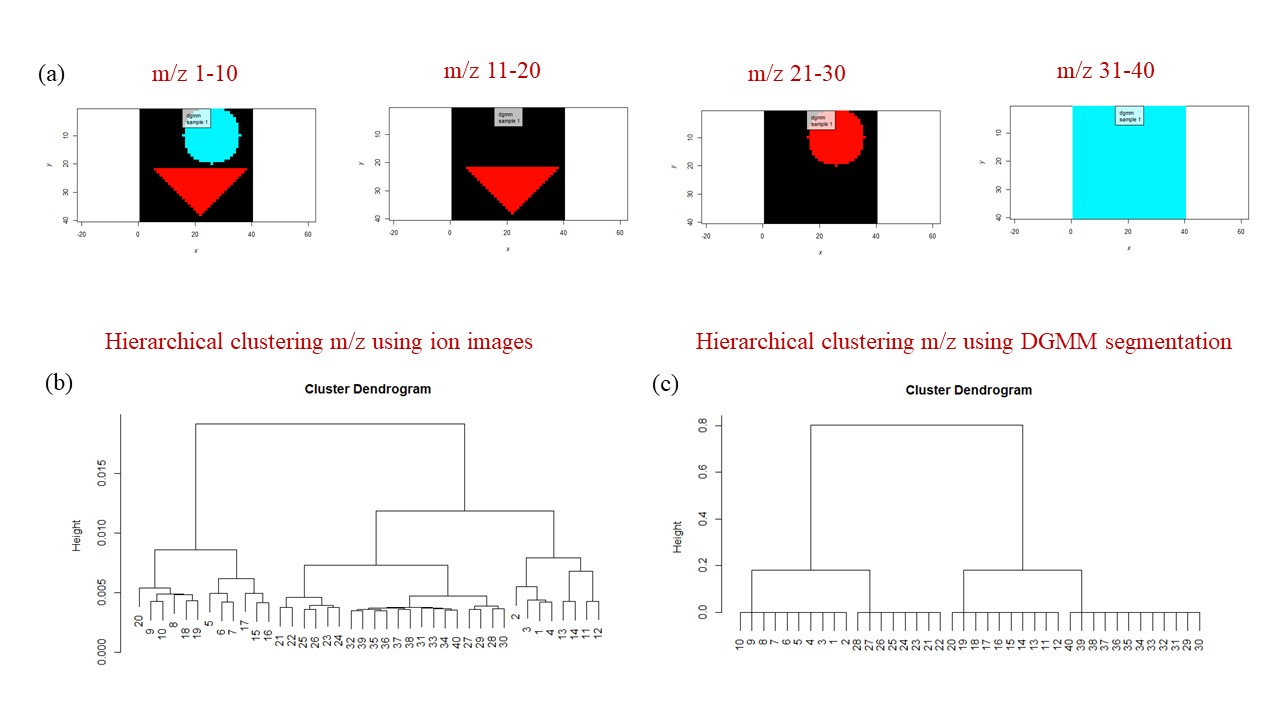
\includegraphics[width=0.8\textwidth]{figure7.jpg}
    \caption{clustering based on ion image and morphological component generated by DGMM}
    \label{fig:figure7}
\end{figure}
\citealp{Boffelli03} might want to know about text text text
text\vspace*{1pt}

Clustering pixels of similar molecular profiles using whole mass spectrum has been studied using spatial aware K-means and spatial centroid segmentation method. However clustering $m/z$s of similar spatial patterns have not been well studied. A naive way of doing this is to cluster $m/z$s based on the Euclidien distance between vectors of ion images. However the spatial information will be lost and it's very sensitive to the ion intensity. In Fig XXX, the simulated ion images of $m/z$ 1-10, 11-20, 21-30, 31-40 have identical spatial patterns respectively. The results of clustering based on Euclidien distance between vectors of ion images show that $m/z$s within each cluster do not have the same spatial patterns. FIg XX shows the results of clustering $m/z$s based on the Dice distance between vectors of morphological component labels and we can see that $m/z$s within the same cluster have identical spatial patterns.

\subsection{Morphological Component-Wise statistical analysis}


\begin{itemize}
\item problems of averaging statistical analysis
\item advantage of Morphological Component-Wise statistical analysis
\item state of concept: real data example and simulation
\end{itemize}









%%%%%%%%%%%%%%%%%%%%%%%%%%%%%%%%%%%%%%%%%%%%%%%%%%%%%%%%%%%%%%%%%%%%%%%%%%%%%%%%%%%%%
%
%     please remove the " % " symbol from \centerline{\includegraphics{fig01.eps}}
%     as it may ignore the figures.
%
%%%%%%%%%%%%%%%%%%%%%%%%%%%%%%%%%%%%%%%%%%%%%%%%%%%%%%%%%%%%%%%%%%%%%%%%%%%%%%%%%%%%%%






\section{Conclusion}

(Table~\ref{Tab:01}) Text Text Text Text Text Text  Text Text Text
Text Text Text Text Text Text  Text Text Text Text Text Text.
Figure~2\vphantom{\ref{fig:02}} shows that the above method  Text
Text Text Text  Text Text Text Text Text Text  Text Text.
\citealp{Boffelli03} might want to know about  text text text text
Text Text Text Text Text Text  Text Text Text Text Text Text Text
Text Text  Text Text Text Text Text Text.
Figure~2\vphantom{\ref{fig:02}} shows that the above method  Text
Text Text Text  Text Text Text Text Text Text  Text Text.
\citealp{Boffelli03} might want to know about  text text text text
Text Text Text Text Text Text Text Text Text Text Text Text Text
Text Text  Text Text Text Text Text Text.
Figure~2\vphantom{\ref{fig:02}} shows that the above method  Text
Text Text Text  Text Text Text Text Text Text  Text Text.



Text Text Text Text Text Text  Text Text Text Text Text Text Text
Text Text  Text Text Text Text Text Text.
Figure~2\vphantom{\ref{fig:02}} shows that the above method  Text
Text Text Text  Text Text Text Text Text Text  Text Text.
\citealp{Boffelli03} might want to know about  text text text text

\begin{enumerate}
\item this is item, use enumerate
\item this is item, use enumerate
\item this is item, use enumerate
\end{enumerate}

Text Text Text Text Text Text Text Text Text Text Text Text Text
Text Text Text Text Text Text Text Text.
Figure~2\vphantom{\ref{fig:02}} shows\vadjust{\pagebreak} that the
above method  Text Text Text Text Text Text Text Text Text Text
Text Text.  \citealp{Boffelli03} might want to know about text
text text text Text Text Text Text Text Text  Text Text Text Text
Text Text Text Text Text Text Text Text Text Text Text.
Figure~2\vphantom{\ref{fig:02}} shows that the above method  Text
Text Text Text Text Text Text Text Text Text  Text Text.
\citealp{Boffelli03} might want to know about text text text text
Text Text Text Text Text Text  Text Text Text Text Text Text Text
Text Text Text Text Text Text Text\break Text.


Text Text Text Text Text Text  Text Text Text Text Text Text Text
Text Text  Text Text Text Text Text Text.
Figure~2\vphantom{\ref{fig:02}} shows that the above method  Text
Text Text Text\vspace*{-10pt}


\section*{Acknowledgements}

Text Text Text Text Text Text  Text Text.  \citealp{Boffelli03} might want to know about  text
text text text\vspace*{-12pt}

\section*{Funding}

This work has been supported by the... Text Text  Text Text.\vspace*{-12pt}

%\bibliographystyle{natbib}
%\bibliographystyle{achemnat}
%\bibliographystyle{plainnat}
%\bibliographystyle{abbrv}
%\bibliographystyle{bioinformatics}
%
%\bibliographystyle{plain}
%
%\bibliography{Document}


\begin{thebibliography}{}

\bibitem[Bofelli {\it et~al}., 2000]{Boffelli03}
Bofelli,F., Name2, Name3 (2003) Article title, {\it Journal Name}, {\bf 199}, 133-154.

\bibitem[Bag {\it et~al}., 2001]{Bag01}
Bag,M., Name2, Name3 (2001) Article title, {\it Journal Name}, {\bf 99}, 33-54.

\bibitem[Yoo \textit{et~al}., 2003]{Yoo03}
Yoo,M.S. \textit{et~al}. (2003) Oxidative stress regulated genes
in nigral dopaminergic neurnol cell: correlation with the known
pathology in Parkinson's disease. \textit{Brain Res. Mol. Brain
Res.}, \textbf{110}(Suppl. 1), 76--84.

\bibitem[Lehmann, 1986]{Leh86}
Lehmann,E.L. (1986) Chapter title. \textit{Book Title}. Vol.~1, 2nd edn. Springer-Verlag, New York.

\bibitem[Crenshaw and Jones, 2003]{Cre03}
Crenshaw, B.,III, and Jones, W.B.,Jr (2003) The future of clinical
cancer management: one tumor, one chip. \textit{Bioinformatics},
doi:10.1093/bioinformatics/btn000.

\bibitem[Auhtor \textit{et~al}. (2000)]{Aut00}
Auhtor,A.B. \textit{et~al}. (2000) Chapter title. In Smith, A.C.
(ed.), \textit{Book Title}, 2nd edn. Publisher, Location, Vol. 1, pp.
???--???.

\bibitem[Bardet, 1920]{Bar20}
Bardet, G. (1920) Sur un syndrome d'obesite infantile avec
polydactylie et retinite pigmentaire (contribution a l'etude des
formes cliniques de l'obesite hypophysaire). PhD Thesis, name of
institution, Paris, France.

\end{thebibliography}
\end{document}
